\newchapter{Validierung}
\label{kap:6}


In diesem Kapitel wollen wir numerische Beispiele für das Hindernis- bzw. Kontaktproblem diskutieren. Dabei werden Auswertungen, die aus dem Quellcode aus Anhang \ref{anhang:D} resultieren, benutzt.

Mögliche numerische Beispiele wurden aus den Veröffentlichungen \cite{SiebVee}, \cite{BraeCar}, \cite{BraeCar2} und \cite{CarWri} entnommen.


\section{Numerische Beispiele zum Hindernisproblem}
\label{kap:6.1}

\begin{bsp}[glatte, rotationssymmetrische Lösung]\label{bsp:6.1}
Wir betrachten das Hindernisproblem mit dem Hindernis $\psi \equiv 0$ und der Lastfunktion $f\equiv -2$ auf $\Omega = [-\frac 32,\frac 32]^2$. Die Dirichlet-Randbedingungen\index{Randbedingungen!Dirichlet} werden durch die Funktion
\[
	\tilde u(x,y) = \frac{x^2+y^2}2-\frac 12 \ln(x^2+y^2)-\frac 12
\]
gegeben. Für dieses Problem existiert eine exakte (glatte) Lösung, die in \idx{Polarkoordinaten} wie folgt lautet:
\begin{align}\label{eq:6.1}
	u(r,\varphi) = \begin{cases}
					\frac{r^2}2-\ln (r)-\frac 12 & , r \ge 1 \\
					0 & , \, \text{sonst}
				\end{cases} \, .
\end{align}
Damit lässt sich der exakte Wert des Energiefunktionals $J(u)$ mit \eqref{eq:6.1} ermitteln. Hierfür nutzen wir die Rotationssymmetrie von $u$ aus, da $u$ unabhängig vom Drehwinkel $\varphi$ ist. Dadurch reicht es aus, die zu berechnenden Integrale nur im ersten Quadranten von $\Omega$ zu berechnen. Um jetzt $J(u)= \frac 12 a(u,u)-(f,u)$ zu bestimmen, müssen wir mit der Kettenregel den Zusammenhang zwischen $u_x,u_y$ und $u_r,u_\varphi$ ermitteln. Dieser ergibt sich zu
\begin{align}\label{eq:6.2}
	\begin{pmatrix} u_x \\ u_y \end{pmatrix} = \frac 1r \begin{pmatrix} r \cos \varphi & -\sin\varphi \\ r \sin\varphi & \cos\varphi \end{pmatrix} \begin{pmatrix} u_r \\ r_\varphi \end{pmatrix}.
\end{align}

Da $u_\varphi = 0$ und $u_r = r-\frac 1r$ gilt, erhalten wir für den exakten Wert des Energiefunktionals unter Verwendung von \eqref{eq:6.2}
\begin{align*}
	J(u) & = \frac 12 \int_\Omega \underbrace{\nabla u \nabla u}_{=u_x^2+u_y^2} \, dx dy - \int_\Omega f u \, dx dy \\
	& = 4  \( \frac 12 \int_0^{\frac \pi4} \int_1^{\frac 3{2\cos\varphi}} (\cos^2\varphi + \sin^2\varphi) \(r-\frac 1r\)^2 r \, dr d\varphi  \right. \\
	& \quad + \frac 12 \int_{\frac \pi4}^{\frac {3\pi}4} \int_1^{\frac 3{2\sin\varphi}} (\cos^2\varphi + \sin^2\varphi) \(r-\frac 1r\)^2 r \, dr d\varphi \\
	&\quad  +  2 \int_0^{\frac \pi4} \int_1^{\frac 3{2\cos\varphi}} \(\frac{r^2}2 - \ln(r) - \frac 12\) r \, dr d\varphi  \\
	&\quad  + \left. 2 \int_{\frac \pi4}^{\frac {3\pi}4} \int_1^{\frac 3{2\sin\varphi}} \(\frac{r^2}2 - \ln(r) - \frac 12\) r \, dr d\varphi \) \\
	& \approx 3,980995748730258 \, .
\end{align*}
Die oberen Grenzen $\frac 3{2\cos\varphi}$ und $\frac 3{2\sin\varphi}$ kommen dabei durch Beschreibung der Randpunkte von $\Omega$ in Polarkoordinaten für $\varphi\in [0,\frac\pi4]$  zustande. Die Rotationssymmetrie kann auf das zweite Integral nur deshalb angewendet werden, weil $f$ eine konstante (und damit auch rotationssymmetrische) Funktion ist.


\begin{figure}[h]
\begin{center}
\subfigure[Exakte Lösung für das Hindernisproblem]{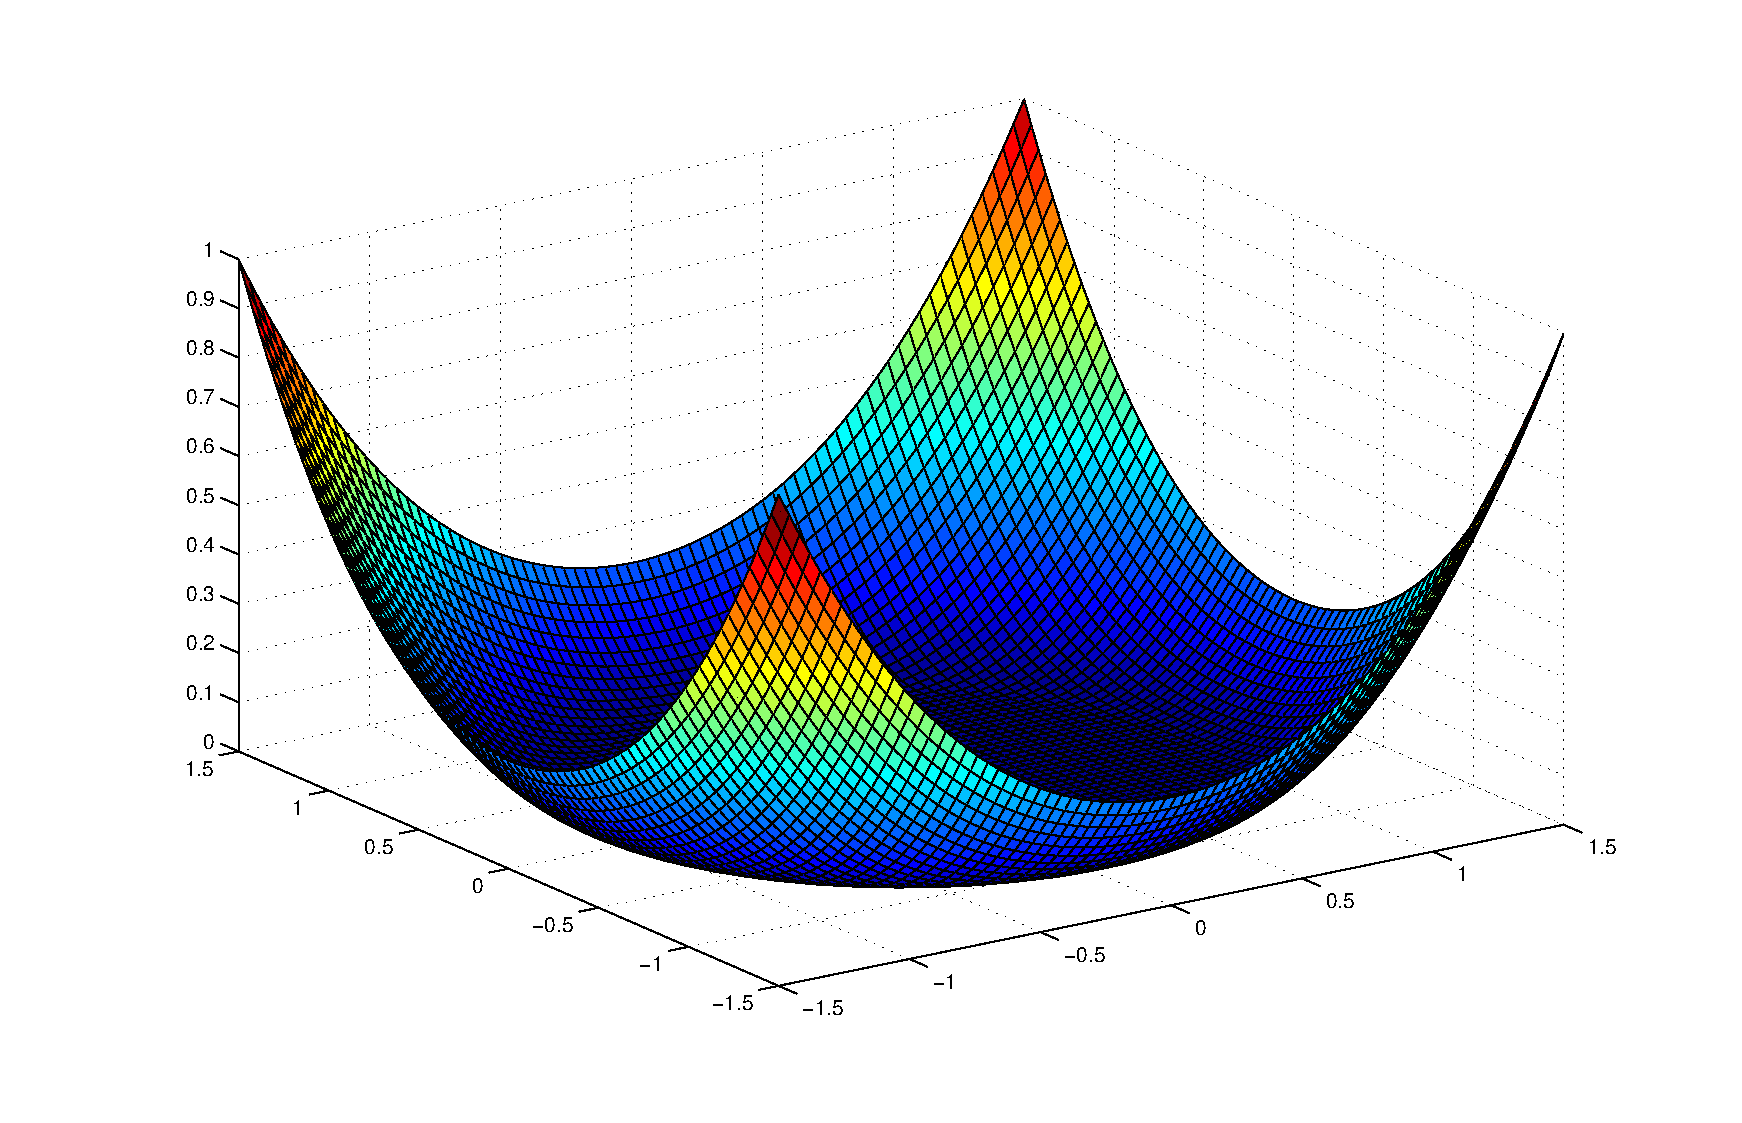
\includegraphics[width=6.25cm]{Abbildungen/exakte_loesung_hindernisproblem1.eps}}
\hfill
\subfigure[Numerische Lösung in der Verfeinerungsstufe 6 mit $\theta_1=0,4$ und $\theta_2=0,3$]{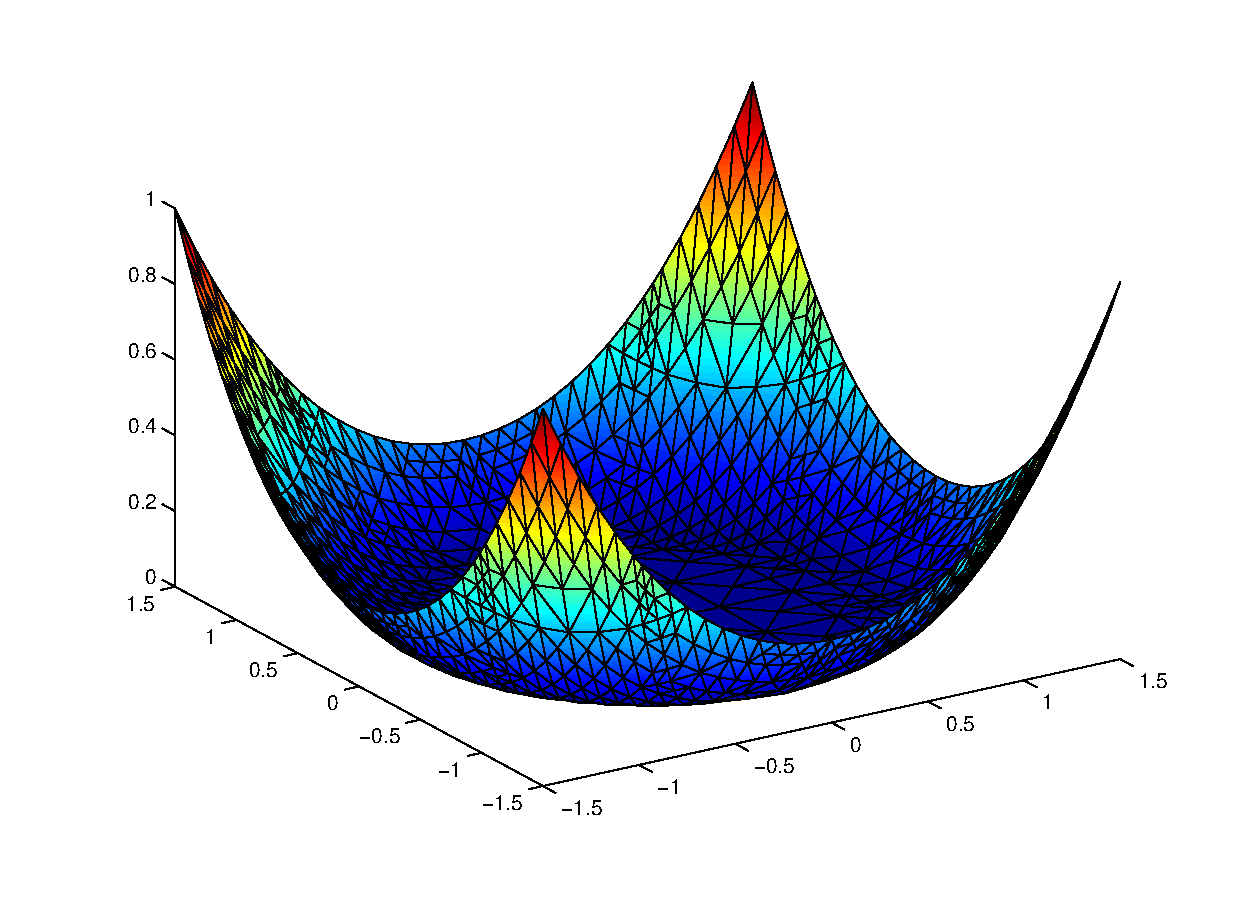
\includegraphics[width=6.25cm]{Abbildungen/num_loesung_bsp1_rec6_0,6_0,5.eps}}
\end{center}
\caption{Exakte und numerische Lösung des Beispiels \ref{bsp:6.1}\label{abb:6.1}}
\end{figure}


\begin{figure}[h]
\begin{center}
\subfigure[Verfeinerungsstufe 6]{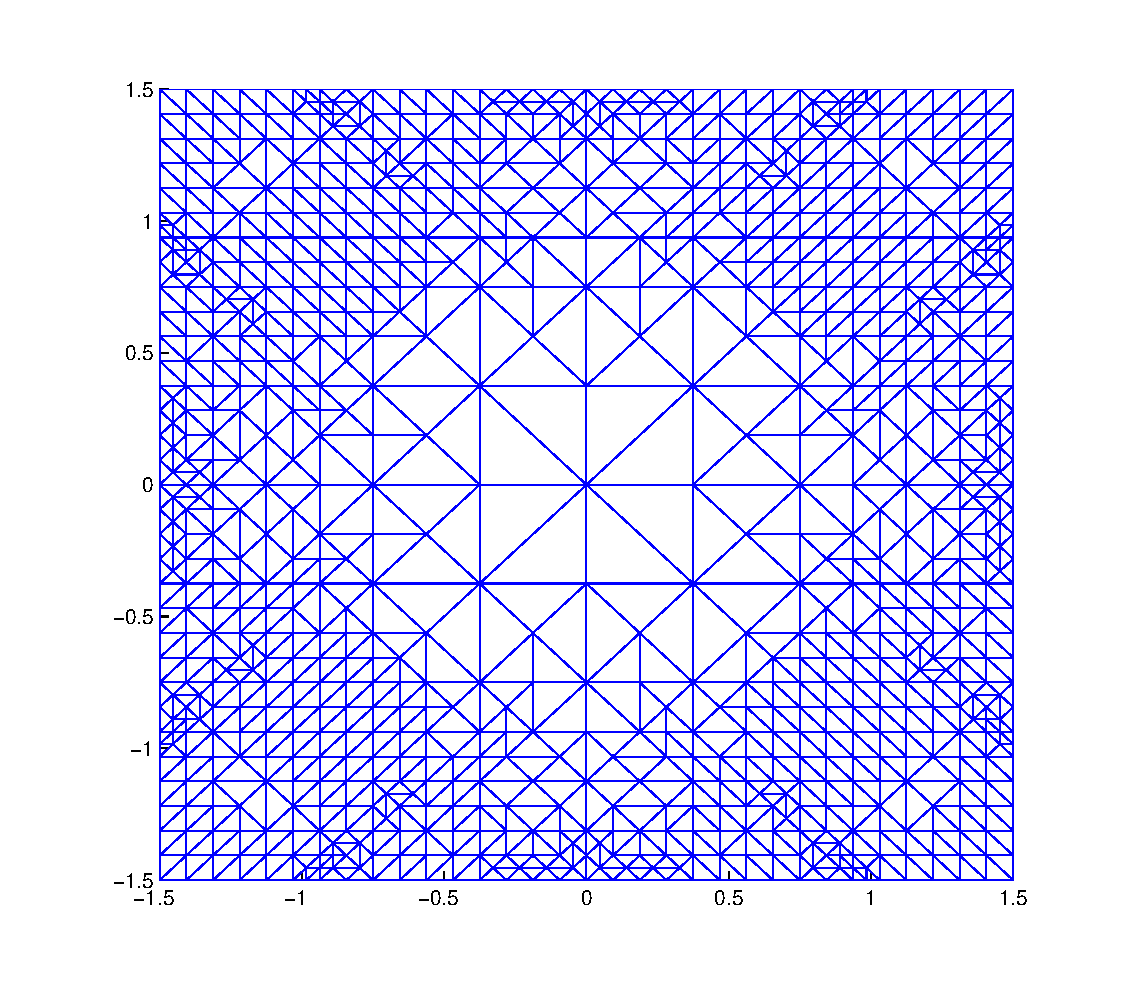
\includegraphics[width=6.2cm]{Abbildungen/mesh_rec6_bsp1.eps}}
\hfill
\subfigure[Verfeinerungsstufe 8]{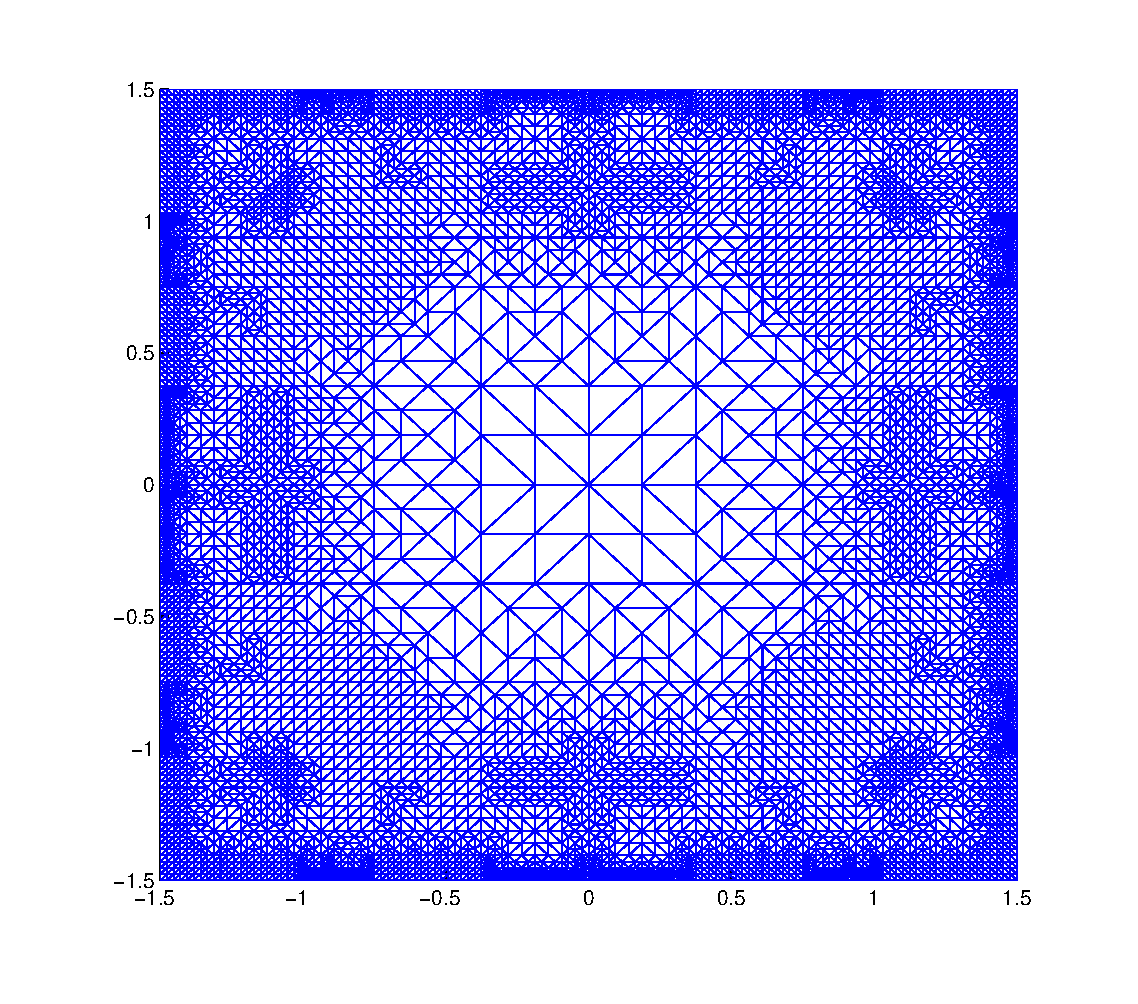
\includegraphics[width=6.25cm]{Abbildungen/mesh_rec8_bsp1.eps}}
\end{center}
\caption{Gitterverfeinerung für das Hindernisproblem im Beispiel \ref{bsp:6.1} mit $\theta_1=0,4$ und $\theta_2=0,3$\label{abb:6.2}}
\end{figure}

In Abbildung \ref{abb:6.1} ist die exakte Lösung die Galerkin-Lösung auf der Verfeinerungsstufe 6 der implementierten, adaptiven Verfeinerungsstrategie im Vergleich dargestellt. In der Tabelle \ref{tab:6.1} sind die Ergebnisse für das Beispiel für $\theta_1 = 0,3$ und $\theta_2 = 0,2$, sowie für eine uniforme Verfeinerung dargestellt. Die maximale Anzahl der Knoten $\abs{\mcal N}$ ist jeweils mittels der Implementierung auf 150.000 begrenzt. Man kann gut erkennen, dass die Anzahl der Knoten im uniformen Fall wesentlich schneller ansteigt. Da in den ersten Verfeinerungsstufen sehr wenig Knoten vorhanden sind, gleichen sich zunächst die adaptive und uniforme Verfeinerung. Der starke Anstieg des Freiheitsgrades in den letzten beiden Schritten liegt daran, dass die lokalen Anteile vom Fehlerindikator $\rho_{\mcal S}$ sehr klein werden (wegen hoher Knotenanzahl) und könnte man durch eine variable Wahl der Parameter $\theta_1$ und $\theta_2$ verringern. 

Weiter stellen wir in Abbildung \ref{abb:6.2} eine adaptive Gitterverfeinerung für das Beispiel \ref{bsp:6.1}, die mit {\ttfamily start_example_1.m} für $\theta_1 = 0,4$ und $\theta_2 = 0,3$ erzeugt werden können, in den Stufen 6 und 8 dar und können gut erkennen, dass im Bereich des vollen Kontaktes weniger stark verfeinert wird. Weiter kann man schön sehen, dass durch die Option {\ttfamily 'symmetric'} das Gitter auch symmetrisch angeordnet bleibt von Verfeinerungsschritt zu Verfeinerungsschritt.


\begin{table}[h]
\centering
\begin{tabular}[c]{|c|c|c|c|c|c|c|c|}
	\hline
	 & \multicolumn{4}{c|}{Adaptive Verfeinerung} & \multicolumn{2}{c|}{Uniforme Verfeinerung} \\
	\hline
	Stufe & $\abs{\mcal N}$ & $\rho_{\mcal S}(\eps_{\mcal V})$ & $-\mcal I_{\mcal Q} (\eps_{\mcal V})$ & $-\mcal I(e)$ & $\abs{\mcal N}$ & $-\mcal I (e)$ \\
	\hline
	 1 &  9  & 6.3512 & 3.1756 & 4.6323 & 9  & 4.6323 \\
	 2 & 25 & 1.8284 & 0.9142 & 1.0978 & 25 & 1.0978 \\
	 3 & 81 & 0.8642 & 0.4349 & 0.2667 & 81 & 0.2667 \\
	 4 & 197 & 0.5422 &0.2713 & 0.1113 & 289 & 0.0670 \\
	 5 & 357 & 0.3896 & 0.1949 & 0.0564 & 1089 &0.0167  \\
	 6 & 821 & 0.2564 & 0.1282 & 0.0231 &4225 &  0.0046 \\
	 7 & 1133 & 0.1896 & 0.0948 & 0.0141 & 16641 & 0.0014 \\
	 8 & 1957 & 0.0993 & 0.0497 & 0.0079 & 66049 & 0.0010 \\
	 9 & 7569 & 0.0476 & 0.0238 & 0.0020 & & \\
	 10 & 29761 & 0.0223 & 0.0112 & 0.0018 & & \\
	 11 & 118017 & 0.0075 & 0.0037 & 0.0007 & & \\
	\hline
\end{tabular}
\caption[Vergleich von adaptiver und uniformer Verfeinerung für Beispiel \ref{bsp:6.1}]{\label{tab:6.1}Vergleich von adaptiver und uniformer Verfeinerung für Beispiel \ref{bsp:6.1} mit Angabe des Freiheitsgrades, a posteriori Fehlerschätzer und exaktem Fehler}
\end{table}


Weiter stellen wir in Abbildung \ref{abb:6.3} auch noch die Oszillationen in einer Verfeinerungsstufe $k$ da. Dabei kann man erkennen, dass es in der Stufe $k=1$ noch einen isolierten Knoten geben muss, der jedoch durch Verfeinerung verschwindet, weil es keinen äquivalenten, isolierten Kontaktpunkt für die exakte Lösung gibt. Außerdem können wir sehen, dass durch die Bedingung aus Lemma \ref{lem:4.24} der Wert der Oszillationsterme von Verfeinerung zu Verfeinerung sinkt.



\begin{figure}[h]
\begin{center}
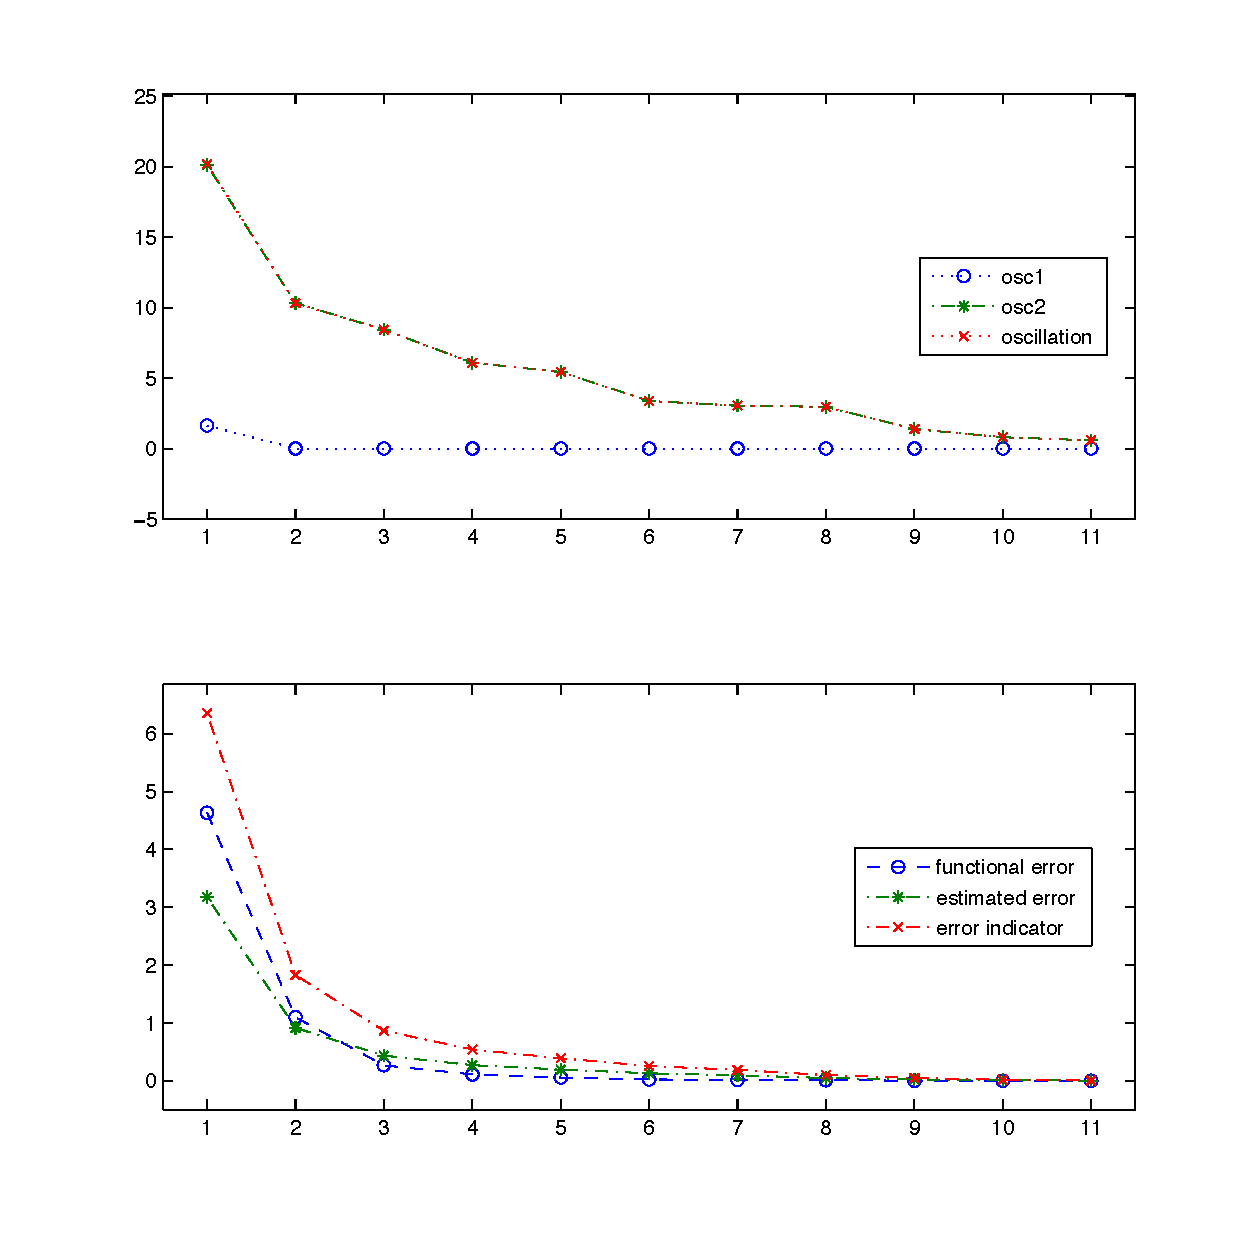
\includegraphics[width=10.5cm]{Abbildungen/adaptive_solution_example1.ps}
\end{center}
\caption[Diagramm mit dem Fehler und der Oszillation für Beispiel \ref{bsp:6.1}]{Oszillationsterme, Fehlerindikator $\rho_{\mcal S}$, Fehlerschätzer $-\mcal I_{\mcal Q}$ und exakten Fehler für Beispiel \ref{bsp:6.1} mit $\theta_1=0,3$ und $\theta_2=0,2$\label{abb:6.3}}
\end{figure}
\end{bsp}


\begin{bsp}[Singularität und L-förmiges Gebiet]\label{bsp:6.2}
Wir wollen nun ein Hindernisproblem mit Singularität im Nullpunkt betrachten, was zu einer starken Verfeinerung an diesem Punkt führen muss. Hierfür sei das Gebiet L-förmig, also von der Form
\[
	\Omega \coloneqq (-2,2)^2 \setminus ([0,2]\times [-2,0]) \, .
\]
Das Hindernis sei wieder durch $\psi \equiv 0$ gegeben und die Lastfunktion in Polarkoordinaten $(r,\varphi)$ durch
\[
	f(r,\varphi) \coloneqq -r^{\frac 23} \sin \(\frac{2\varphi}3\)\(\frac{\gamma_1'(r)}r + \gamma_1''(r)\) - \frac 43r^{\frac 13} \gamma_1'(r) \sin \(\frac{2\varphi}3\)-\gamma_2(r) \, ,
\]
wobei mit $\bar r = 2\(r-\frac 14\)$ gilt
\begin{align*}
	\gamma_1(r) &= \begin{cases}
					1 & , \bar r < 0 \\
					-6\bar r^5+15 \bar r ^4-10 \bar r ^3+1 & , 0 \le \bar r < 1 \\
					0 & , \bar r \ge 1
				\end{cases} \, , \\
	\gamma_2(r) & = \begin{cases}
						0 & , r < \frac 5 4 \\
						1 & , \, \text{sonst}
					\end{cases} \, .
\end{align*}
Für dieses Problem gibt es eine exakte Lösung, die Polarkoordinaten
\[
	u(r,\varphi) = r^{\frac 23} \gamma_1(r)\sin \(\frac{2\varphi}3\) 
\]
lautet. Die Funktion hat im Ursprung eine Singularität. Damit können wir auch für dieses Beispiel mit den Umformungen aus \eqref{eq:6.2} den exakten Wert des Energiefunktionals $J$ berechnen. Durch Anwendung der Polarkoordinaten und Transformationssatz der Integration erhalten wir
\[
	J(u) \approx 0,5 \, .
\]

\textbf{Hier kommen noch die Auswertungen der Daten rein!}

\begin{figure}[h]
\begin{center}
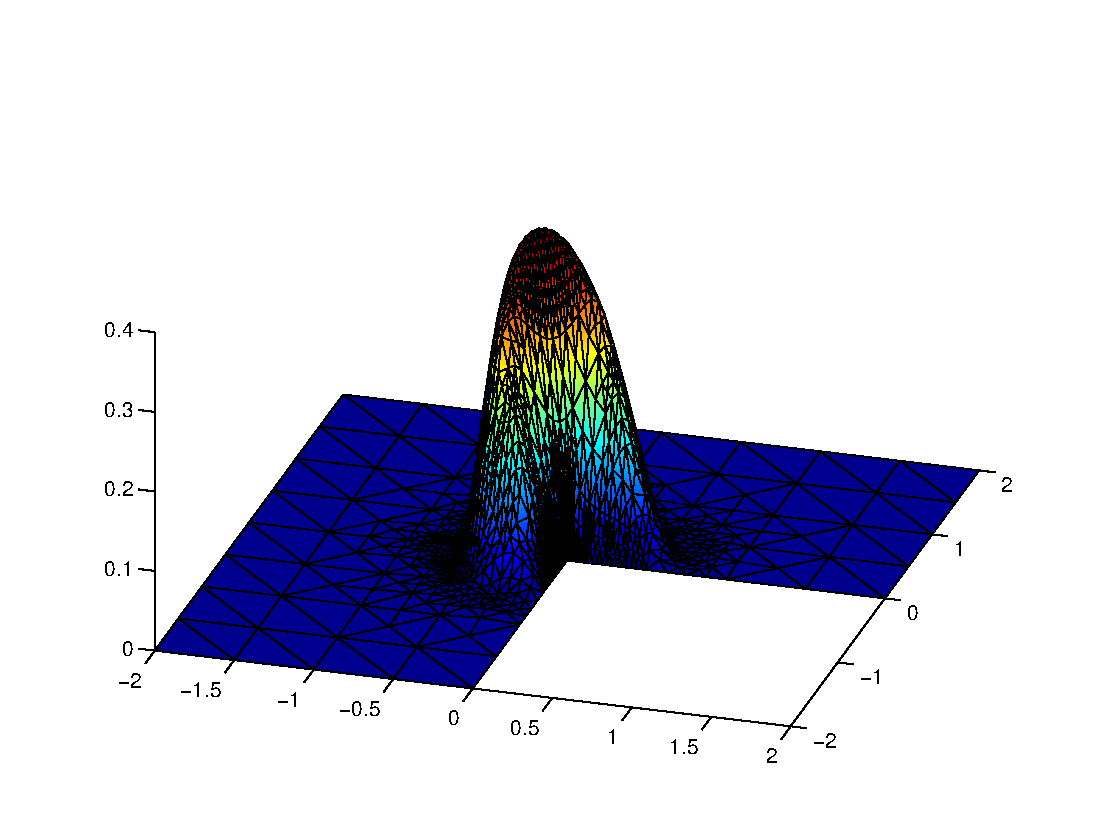
\includegraphics[width=13cm]{Abbildungen/num_loesung_rec7_bsp2.eps}
\end{center}
\caption{Numerische Lösung des Beispiels \ref{bsp:6.2} in der Verfeinerungsstufe 7 mit $\theta_1=\theta_2 = 0,3$}
\end{figure}

\begin{figure}[h]
\begin{center}
\subfigure[Verfeinerungsstufe 6]{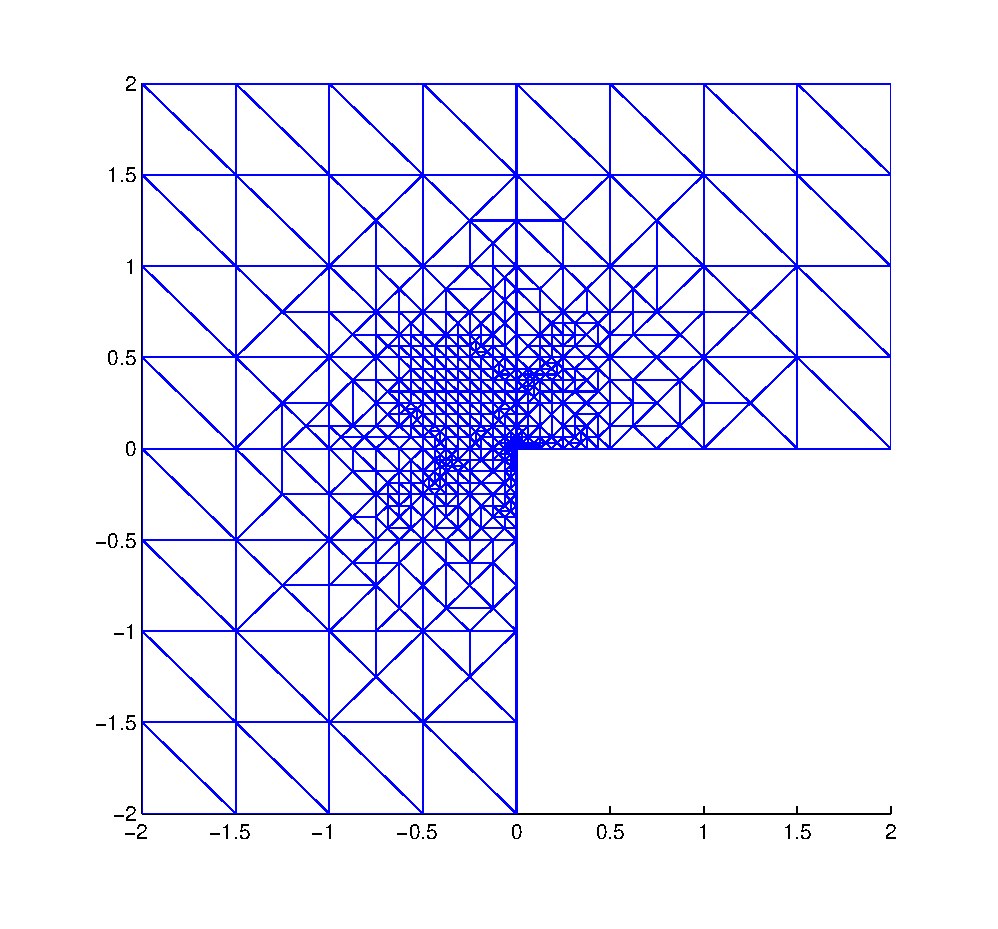
\includegraphics[width=6.26cm]{Abbildungen/mesh_rec6_bsp2.eps}}
\hfill
\subfigure[Verfeinerungsstufe 8]{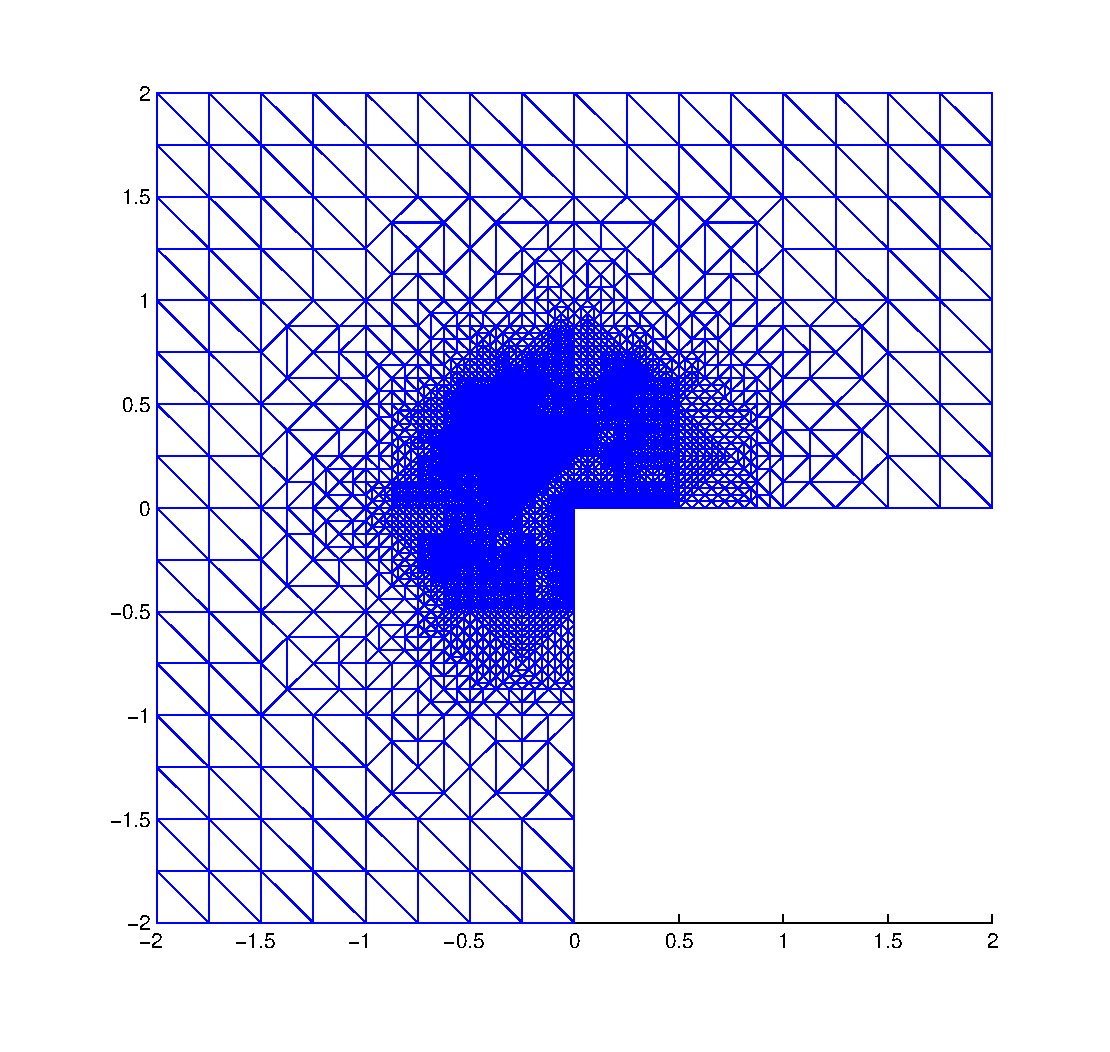
\includegraphics[width=6.26cm]{Abbildungen/mesh_rec8_bsp2.eps}}
\end{center}
\caption{Netzverfeinerungen für das Beispiel \ref{bsp:6.2} mit $\theta_1=\theta_2=0,3$}
\end{figure}
\end{bsp}

\begin{bsp}\label{bsp:6.3}
Als letztes Beispiel für ein affines Hindernisproblem können wir das Beispiel \ref{bsp:6.2} noch erweitern, indem wir als affines Hindernis nicht die Nullfunktion, sondern eine umgedrehte Pyramide verwenden, die gegeben wird durch
\[
	\psi (x) \coloneqq 0,5 \,  (\dist (x,\partial [-2,2]^2)-2,01) \, , \quad x \in \bar \Omega \, .
\]

\textbf{Hier kommen noch die Auswertungen der Daten rein!}


\begin{figure}[h]
\begin{center}
\includegraphics[width=13cm]{Abbildungen/num_loesung_bsp3.eps}
\end{center}
\caption{Numerische Lösung des Beispiels \ref{bsp:6.3} mit $\theta_1=\theta_2 = 0,3$}
\end{figure}


\begin{figure}[h]
\begin{center}
\subfigure[Verfeinerungsstufe 6]{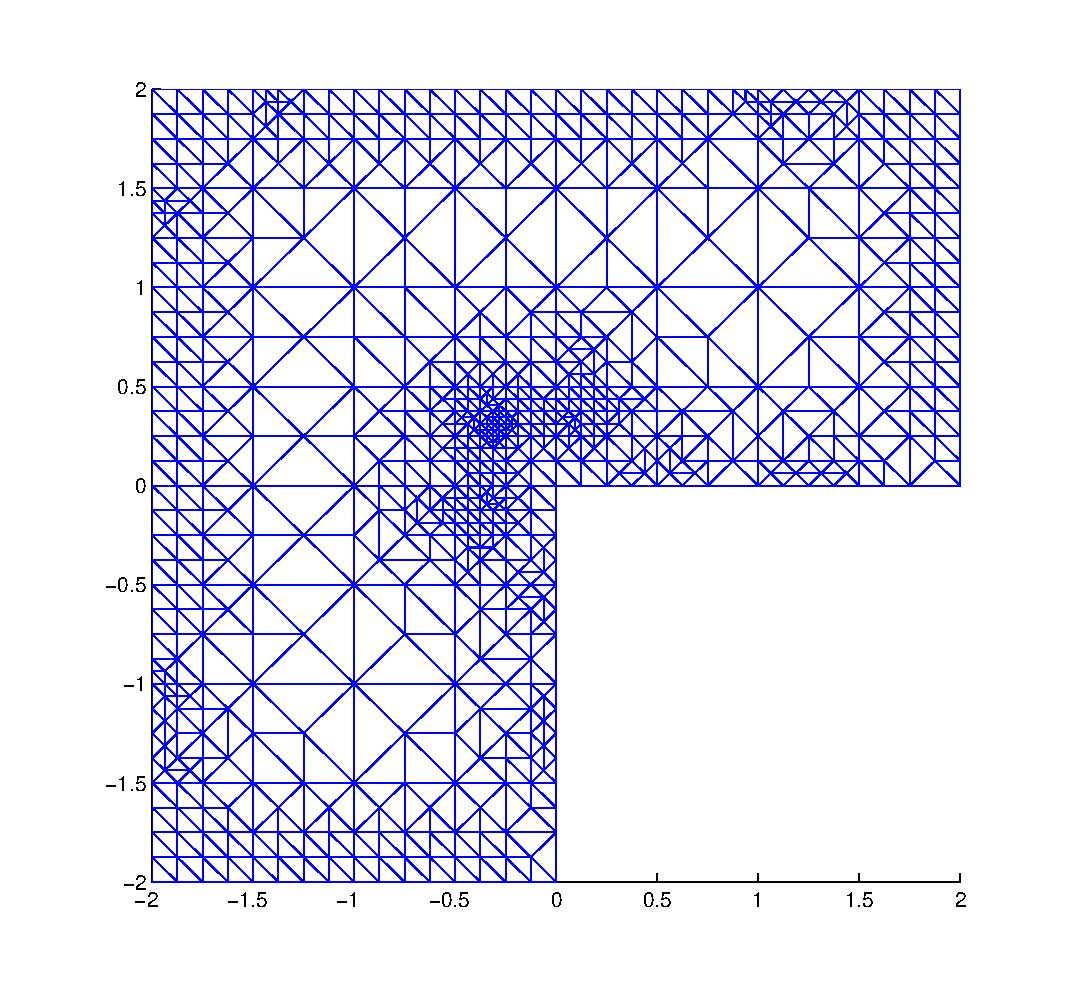
\includegraphics[width=6.26cm]{Abbildungen/mesh_rec6_bsp3.eps}}
\hfill
\subfigure[Verfeinerungsstufe 8]{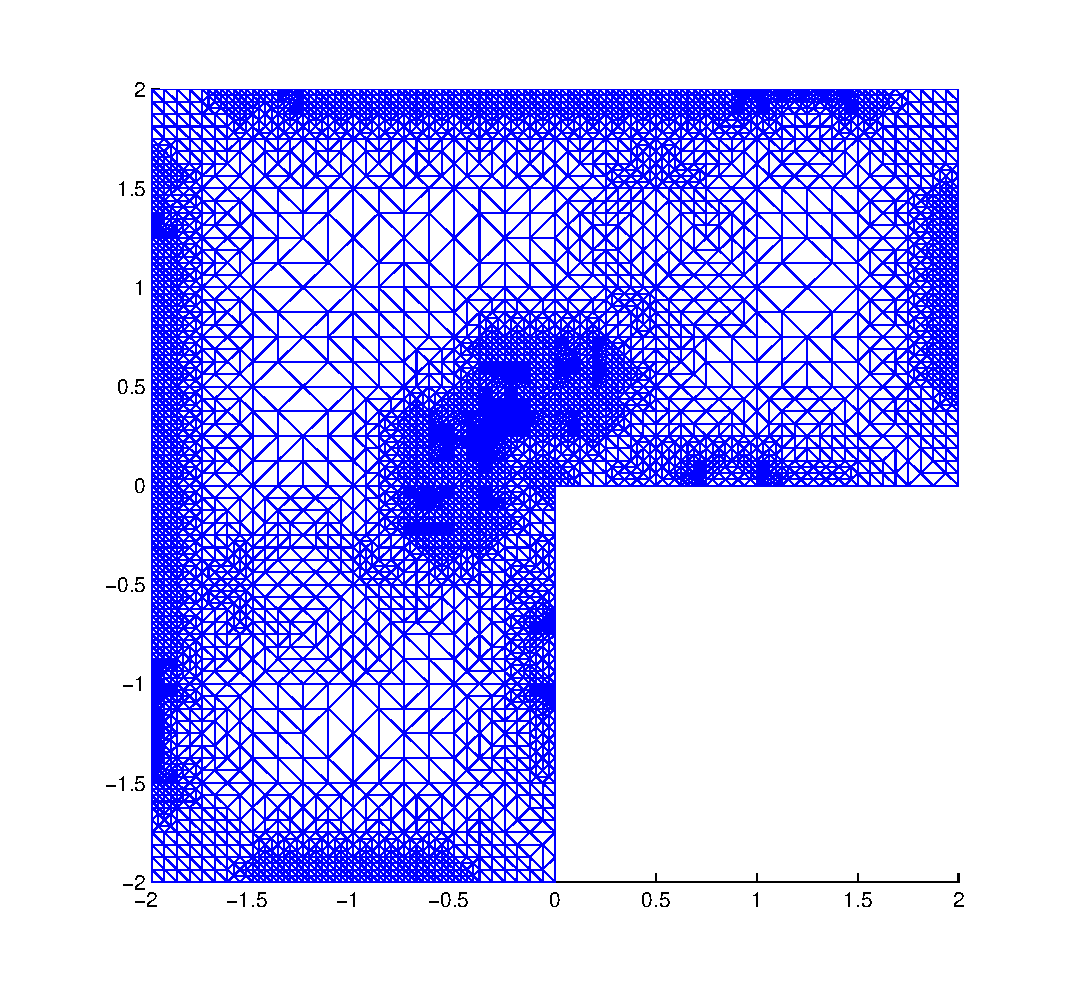
\includegraphics[width=6.26cm]{Abbildungen/mesh_rec8_bsp3.eps}}
\end{center}
\caption{Netzverfeinerungen für das Beispiel \ref{bsp:6.3} mit $\theta_1=\theta_2=0,3$}
\end{figure}
\end{bsp}


\section{Numerisches Beispiel zum Kontaktproblem}
\label{kap:6.2}



\subsubsection{meine Stichpunkte}

\begin{itemize}
\item numerisches Beispiel (Problemstellung) $\ra$ vielleicht mit Kontakt und nur Hindernis
\item Vergleich mit Analytischer Lösung?! (Tabelle mit Ergebnissen) $\ra$ Ergebnisse diskutieren
\end{itemize}


\newpage

%%% Local Variables: 
%%% mode: latex
%%% TeX-master: "Skript"
%%% End: 
